\paragraph{QuizziPedia::Front-End::Views::ClickableAreaQuestionsView}
\begin{figure} [ht]
	\centering
	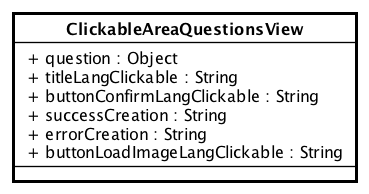
\includegraphics[scale=0.80]{UML/Classi/Front-End/QuizziPedia_Front-end_ClickableAreaQuestionsView.png}
	\caption{QuizziPedia::Front-End::Views::ClickableAreaQuestionsView}
\end{figure} \FloatBarrier
\begin{itemize}
	\item \textbf{Descrizione}: \textit{view\ped{G}} contenente i campi e le direttive per creare una domanda ad area cliccabile;
	\item \textbf{Utilizzo}:  permette all'utente di creare una domanda ad area cliccabile compilando i campi proposti;
	\item \textbf{Relazioni con altre classi}:
	\begin{itemize}
		\item \textbf{IN \texttt{ClickableAreaQuestionsModelView}}: classe di tipo modelview la cui istanziazione è contenuta all'interno della variabile di ambiente \texttt{\$scope} di \textit{Angular\ped{G}}. All'interno di essa sono presenti le variabili e i metodi necessari per il \textit{Two-Way Data-Binding\ped{G}} tra la \textit{view\ped{G}} \texttt{ClickableAreaQuestionsView} e il \textit{controller\ped{G}}\\ \texttt{ClickableAreaQuestionsController};
		\item \textbf{IN \texttt{TopicKeywordsDirective}}: \textit{directive\ped{G}} che permette di gestire l'inserimento di keywords al momento della creazione della domanda;
		\item \textbf{IN \texttt{QuestionTextDirective}}: rappresenta il componente grafico che permette all'utente di scrivere o modificare il testo di una domanda;
		\item \textbf{IN \texttt{LangModel}}: rappresenta il modello delle informazioni per la giusta traduzione dell'applicazione.
	\end{itemize}
	\item \textbf{Attributi}:
	\begin{itemize}
		\item \texttt{+ question: Object} \\ Oggetto contenente gli attributi per la creazione della domanda:
		\begin{itemize}
			\item \texttt{url}: attributo di tipo \texttt{String} che contiene l'\textit{URL\ped{G}} associato all'immagine;
			\item \texttt{answer}: array contenente oggetti che rappresentano le risposte. Ogni oggetto risposta contiene:
			\begin{itemize}
				\item \texttt{x}: attributo di tipo \texttt{Number} che rappresenta la posizione della risposta nell'asse delle ascisse all'interno dell'immagine;
				\item \texttt{y}: attributo di tipo \texttt{Number} che rappresenta la posizione della risposta nell'asse delle ordinate all'interno dell'immagine.
			\end{itemize}
		\end{itemize}	
		\item \texttt{+ titleLangClickable: String} \\ Attributo che viene utilizzato per visualizzare la giusta traduzione del titolo della pagina, in italiano o in inglese;
		\item \texttt{+ buttonConfirmLangClickable: String} \\ Attributo che viene utilizzato per visualizzare la giusta traduzione della \textit{label\ped{G}} per il bottone di conferma, in italiano o in inglese;
		\item \texttt{+ buttonLoadImageLangClickable: String} \\ Attributo che viene utilizzato per visualizzare la giusta traduzione della \textit{label\ped{G}} per il bottone di caricamento dell'immagine nel testo della domanda, in italiano o in inglese;
		\item \texttt{+ successCreation: String} \\ Attributo che visualizza un messaggio di conferma avvenuta creazione della domanda;
		\item \texttt{+ errorCreation: String} \\ Attributo che visualizza un messaggio d'errore per la creazione della domanda.
	\end{itemize}
\end{itemize}